\documentclass{article}

\usepackage{graphicx}
\usepackage{tikz}
\usepackage{tikzsymbols}
\usetikzlibrary{calc,patterns,shapes.geometric}
\pagestyle{empty}
\usepackage[margin=0pt]{geometry}
\geometry{papersize={14in,12in}}

\def\centerarc[#1](#2)(#3:#4:#5){\draw[#1] ($(#2)+({#5*cos(#3)},{#5*sin(#3)})$) arc (#3:#4:#5);}

\begin{document}
	\begin{figure}
		\centering
		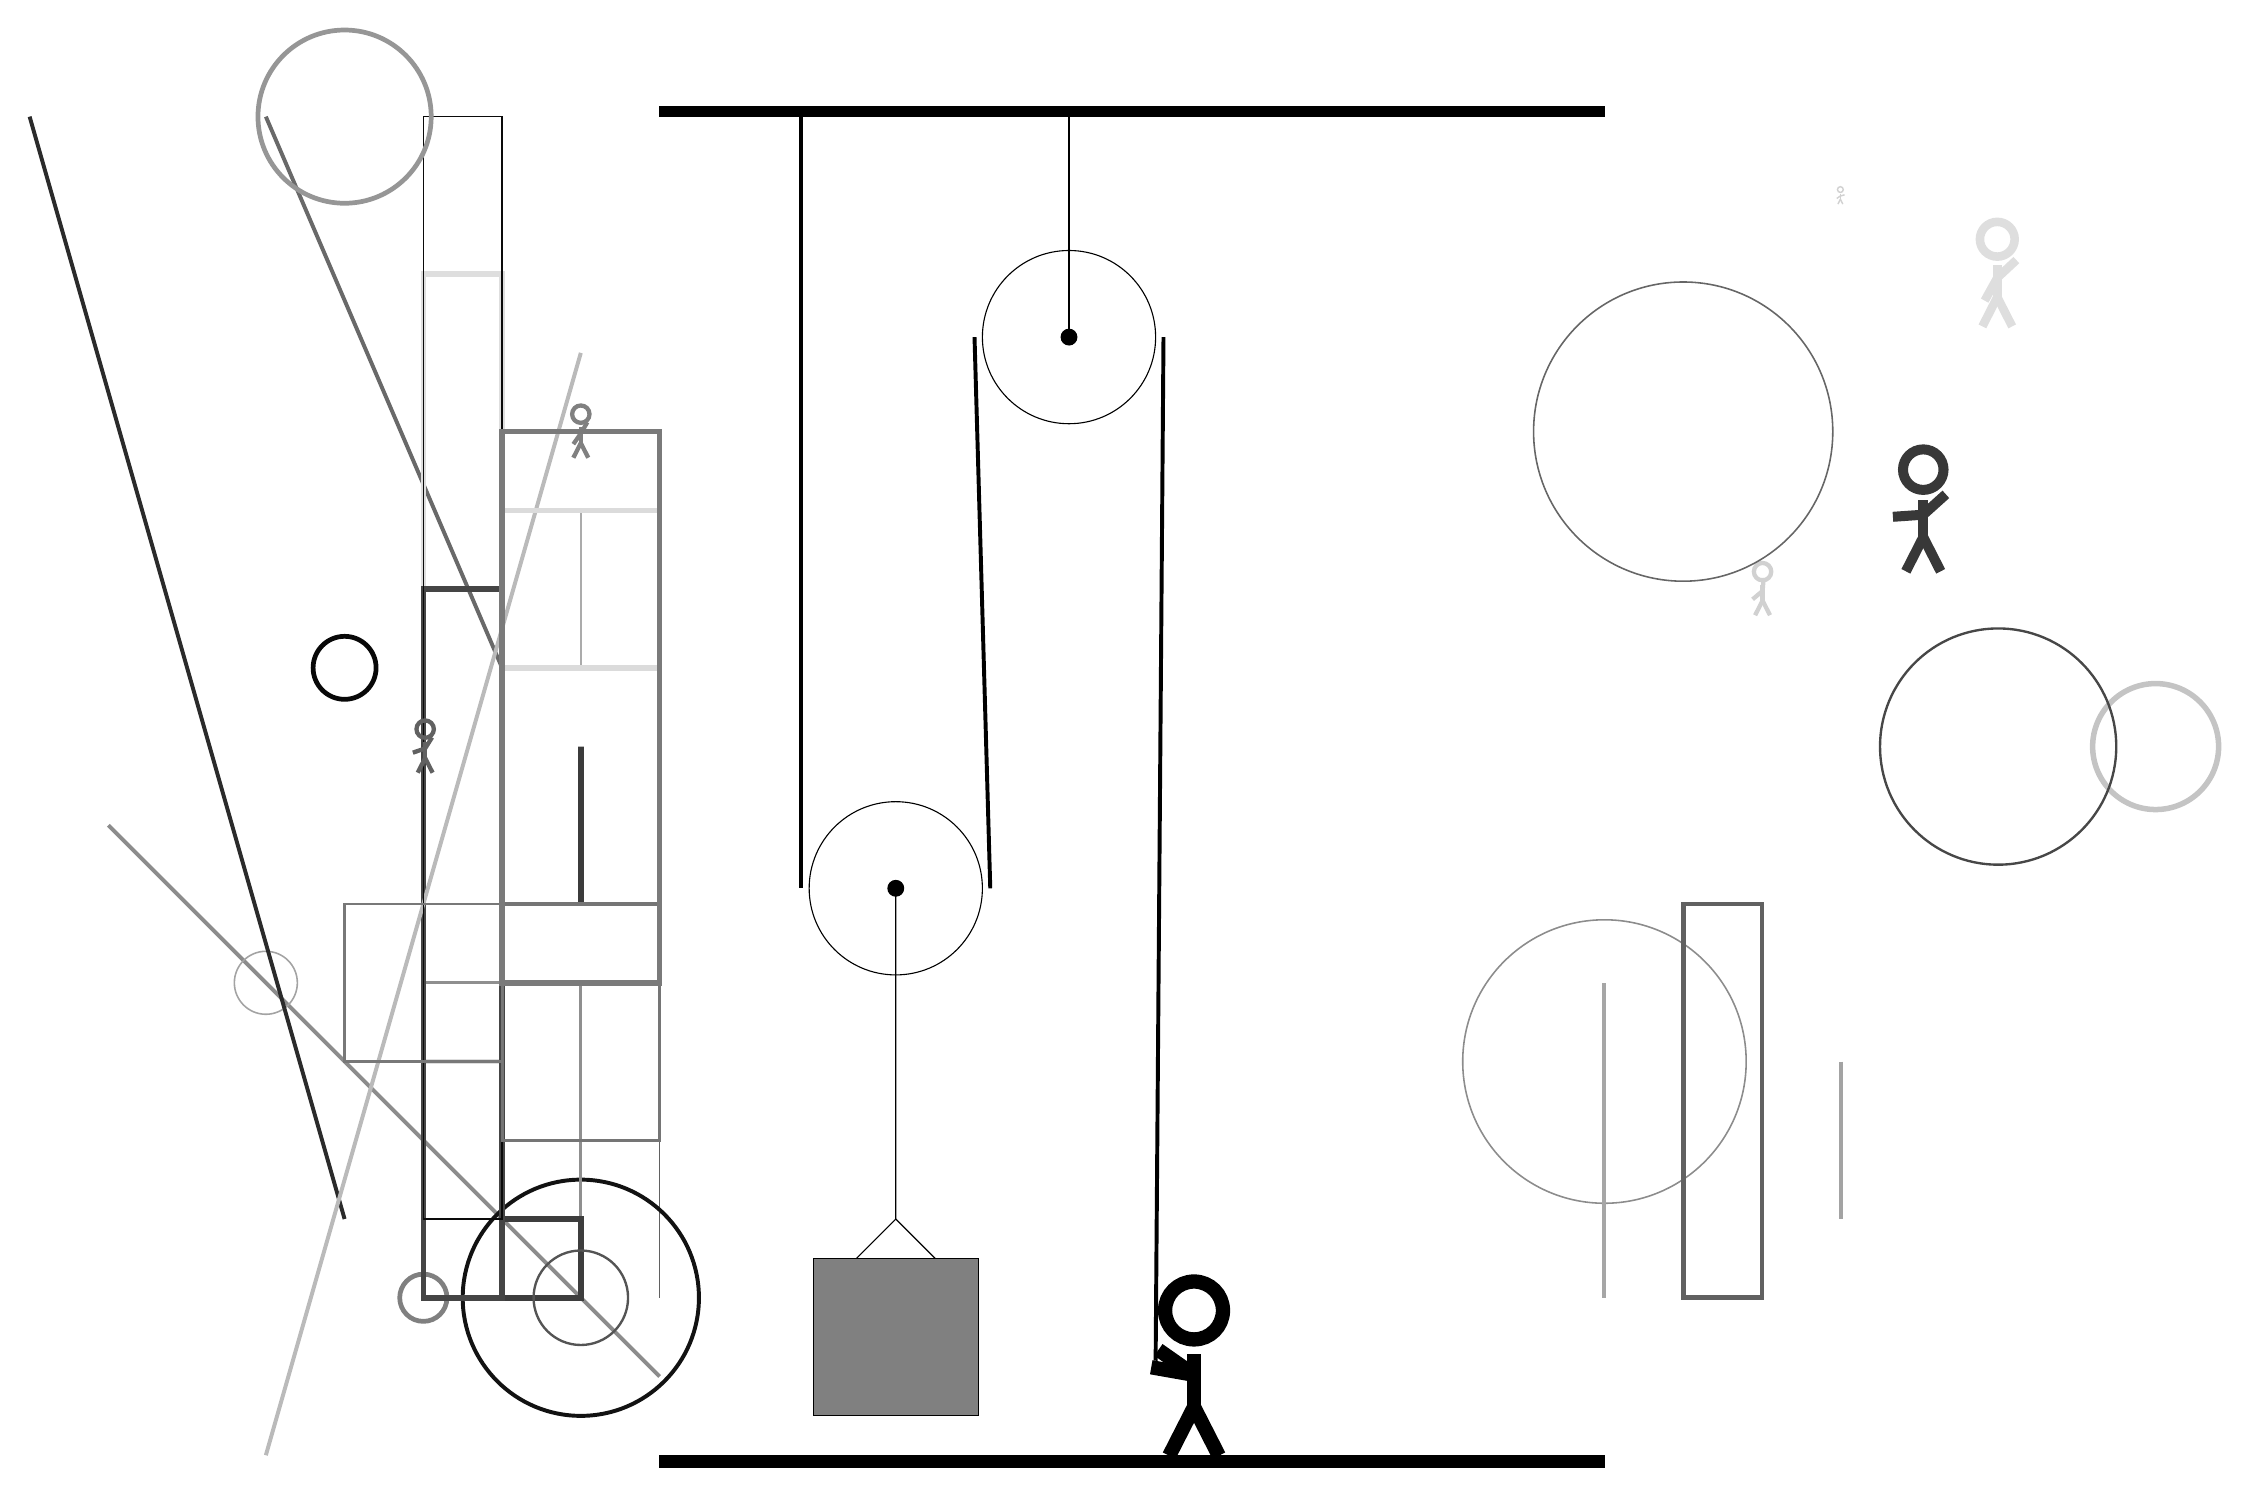
\begin{tikzpicture}
			%%%%% START %%%%%
			
			\draw[fill=black] (-2, 14) rectangle (10, 14.125);
			
			\draw (3.2, 11.2) circle (1.1);
			\draw[fill=black] (3.2, 11.2) circle (0.1);
			\draw[thick] (3.2, 11.2) -- (3.2, 14);
			
			\draw (1, 4.2) circle (1.1);
			\draw[fill=black] (1, 4.2) circle (0.1);
			
			\draw (1, 4.2) -- (1, 0) -- (0.5, -0.5);
			\draw (1, 0) -- (1.5, -0.5);
			\draw[fill=black!50] (-0.05, -0.5) rectangle (2.05, -2.5);
			
			\draw[line width=0.5mm] (-0.2, 14) -- (-0.2, 4.2);
			\centerarc[line width=0.5mm](1, 4.2)(180:360:1.2000000000000002);
			\draw[line width=0.5mm](2.2, 4.2) -- (2.0, 11.2);
			\centerarc[line width=0.5mm](3.2, 11.2)(0:180:1.2000000000000002);
			\draw[line width=0.5mm](4.4, 11.2) -- (4.3, -1.8);
			
			\node at (4.7, -1.9) {\Strichmaxerl[10][-35][170]};
			
			\draw[line width=0.5mm, color=black!36](13, 2) -- (13, 0);
			
			\draw[line width=0.5mm, color=black!59](-4, 7) -- (-7, 14);
			\draw[line width=0.2mm, color=black!62] (-2, 10) rectangle (-2, -1);
			\draw [line width=0.7mm, color=black!23](17, 6) circle (0.8);
			
			\node[line width=0.7mm, color=black!18] at (12, 8) {\Strichmaxerl[3][40][85]};
			
			\draw[line width=0.7mm, color=black!13] (-4, 2) rectangle (-5, 12);
			\node[line width=0.5mm, color=black!50] at (-3, 10) {\Strichmaxerl[3][55][60]};
			\draw[line width=0.5mm, color=black!45](-2, -2) -- (-9, 5);
			\draw [line width=0.2mm, color=black!36](-7, 3) circle (0.4);
			\draw [line width=0.5mm, color=black!93](-3, -1) circle (1.5);
			
			\draw[line width=0.3mm, color=black!33] (-2, 9) rectangle (-3, 7);
			\draw [line width=0.2mm, color=black!45](10, 2) circle (1.8);
			\draw [line width=0.3mm, color=black!72](15, 6) circle (1.5);
			
			\draw[line width=0.4mm, color=black!44] (-3, 3) rectangle (-5, -1);
			\draw [line width=0.6mm, color=black!50](-5, -1) circle (0.3);
			\node[line width=0.5mm, color=black!13] at (15, 12) {\Strichmaxerl[6][61][43]};
			
			\draw[line width=0.5mm, color=black!83](-6, 0) -- (-10, 14);
			\draw[line width=0.7mm, color=black!76] (-3, 0) rectangle (-4, -1);
			\draw[line width=0.7mm, color=black!77] (-3, 4) rectangle (-3, 6);
			
			\node[line width=0.5mm, color=black!78] at (14, 9) {\Strichmaxerl[7][4][42]};
			\draw [line width=0.3mm, color=black!67](-3, -1) circle (0.6);
			\draw[line width=0.7mm, color=black!73] (-4, 8) rectangle (-5, -1);
			\node[line width=0.5mm, color=black!18] at (13, 13) {\Strichmaxerl[1][34][16]};
			\draw[line width=0.5mm, color=black!27](-3, 11) -- (-7, -3);
			\draw [line width=0.6mm, color=black!97](-6, 7) circle (0.4);
			
			\draw[line width=0.2mm, color=black!96] (-4, 14) rectangle (-5, 0);
			
			\draw[line width=0.2mm, color=black!82] (-2, 6) rectangle (-2, 6);
			\draw [line width=0.6mm, color=black!41](-6, 14) circle (1.1);
			\draw[line width=0.4mm, color=black!54] (-2, 1) rectangle (-4, 4);
			\draw[line width=0.6mm, color=black!62] (11, 4) rectangle (12, -1);
			\draw[line width=0.7mm, color=black!14] (-2, 7) rectangle (-4, 9);
			
			\draw[line width=0.3mm, color=black!53] (-4, 4) rectangle (-6, 2);
			\draw [line width=0.2mm, color=black!60](11, 10) circle (1.9);
			
			\node[line width=0.3mm, color=black!62] at (-5, 6) {\Strichmaxerl[3][19][58]};
			\draw[line width=0.5mm, color=black!35](10, -1) -- (10, 3);
			\draw[line width=0.7mm, color=black!52] (-2, 3) rectangle (-4, 10);
			
			\draw[fill=black] (-2, -3) rectangle (10, -3.15);
			
			%%%%% END %%%%%
		\end{tikzpicture}
	\end{figure}	
\end{document}